\subsection{Introduction}
\begin{frame}{Generative models}{Introduction}

\begin{itemize}
    \item Suppose that we wish to classify an observation into one of $K$ classes, where $K \geq 2$. \pause 
    
    \item Let $\pi_K$ represent the \textbf{prior} probability that a randomly chosen observation comes from the prior $k$th class. \pause
    
    \item Let $f_k(X) \equiv  Pr(X|Y = k)$ denote the \textit{density function} of $X$ for an observation that comes from the $k$th class. \\ \pause
    
    $\rightarrow$ $f_k(x)$ is relatively large if there is a high probability that an observation in the $k$th class has $X \approx x$. \\ \pause
    $\rightarrow$ $f_k (x)$ is small if it is very unlikely that an observation in the $k$th class has $X \approx x$. \pause 

    \item Then Bayes’ theorem states that, \pause 


    $$ p_k(x) =  \text{Pr}(Y=k|X=x) = \frac{\pi_k f_k (x)}{  \sum_{l=1}^K \pi_l f_l(x)  }.$$
 
    
\end{itemize}

\end{frame}

\begin{frame}{Generative models}{Introduction}

        \begin{equation}\label{eq:bayes}
           p_k(x) =  \text{Pr}(Y=k|X=x) = \frac{\pi_k f_k (x)}{  \sum_{l=1}^K \pi_l f_l(x)  }. 
        \end{equation}

\begin{itemize}
    
    \item We only need the estimates of $\pi_k$ and $f_k(x).$ \pause 
    \item Estimating $\pi_k$ is easy if we have a random sample from the population. \pause  \\ 
    $\rightarrow $ Compute the fraction of the observations that belong to the $k$th class. \pause
    
    \item Estimating the $f_k(x)$ is much more challenging. \pause
    
    \item As we will see, to estimate $f_k(x)$, we will typically have to make some simplifying assumptions. \pause

    \item We'll discuss three classifiers that use different
estimates of $f_k(x)$: \pause \\ 
    \begin{itemize}
        \item \textit{Linear discriminant analysis}, \pause 
        \item \textit{Quadratic discriminant analysis}, \pause
        \item \textit{Naive Bayes}.
    \end{itemize}
        
\end{itemize}
    
\end{frame}


\subsection{Linear discriminant analysis for $p = 1$}
\begin{frame}{Generative models}{Linear discriminant analysis for $p=1$}

\begin{itemize}
    \item For now, assume that $p=1$: we have only one predictor. \pause
    \item We want to obtain estimates for $f_k(x), \pi_k$ such as we can plug into (\ref{eq:bayes}) in order to estimate $p_k(x)$. \pause
    \item We'll assume that $f_k(x)$ is \textit{normal}, \pause

    \begin{equation}\label{eq:gaussian}
        f_k(x) = \frac{1}{\sqrt{ 2\pi } \sigma_k} \text{exp} \left(  - \frac{1}{2\sigma_k^2} (x - \mu_k)^2    \right)
    \end{equation} \pause

    \item Where $\mu_k$ and $\sigma_k^2$ are the mean and variance parameters for the $k$th class. \pause

    \item We'll assume constant variance so, $\sigma_1^2 = \cdots = \sigma_K^2 = \sigma^$. \pause

    \item Plugging (\ref{eq:gaussian}) into (\ref{eq:bayes}), results \pause

    \begin{equation}\label{eq:linear-prob}
        p_x(x) = \frac{\pi_k \frac{1}{\sqrt{2\pi} \sigma}   \text{exp} \left(  - \frac{1}{2\sigma^2} (x - \mu_k)^2   \right)  }{  \sum_{l=1}^K  \pi_l \frac{1}{\sqrt{2\pi} \sigma}  \text{exp} \left(  - \frac{1}{2\sigma^2} (x - \mu_l)^2 \right) }
    \end{equation}
\end{itemize} 


\end{frame}


\begin{frame}{Generative models}{Linear discriminant analysis for $p=1$}

    \begin{equation*}
        p_x(x) = \frac{\pi_k \frac{1}{\sqrt{2\pi} \sigma}   \text{exp} \left(  - \frac{1}{2\sigma^2} (x - \mu_k)^2    \right)  }{  \sum_{l=1}^K  \pi_l \frac{1}{\sqrt{2\pi} \sigma}   \text{exp} \left(  - \frac{1}{2\sigma^2} (x - \mu_l)^2    \right)       }
    \end{equation*}

\begin{itemize}

    \item Taking the log of (\ref{eq:linear-prob}) and rearranging the terms, \pause

    
    \begin{equation} \label{eq:delta-linear}
        \delta_k(x) = x \cdot \frac{\mu_k}{\sigma^2} - \frac{\mu_k^2}{2 \sigma^2} + \log{(\pi_k)}
    \end{equation} \pause

        \item To apply the Bayes classifier we still have to estimate the parameters $\pi_k$, $\mu_k$ and $\sigma^2$.  

\end{itemize}
    
\end{frame}


\begin{frame}{Generative models}{Linear discriminant analysis for $p=1$}

\begin{itemize}

    \item The following estimates are used: \pause

    \begin{align}
        \hat{\mu}_k &= \frac{1}{n_k} \sum_{i:y_i = k} x_i \\
        \hat{\sigma}^2 &= \frac{1}{n-K} \sum_{k=1}^K \sum_{i:y_i = k} (x_i - \hat{\mu}_k)^2.
    \end{align} \pause

    where $n$ is the total number of training observations, and $n_k$ is the number of training observations in the $k$th class. \pause

\item Sometimes we have knowledge of the class membership probabilities $\pi_1, \cdots, \pi_K $, which can be used directly. \pause

\item In the absence of any additional
information, LDA estimates $\pi_k$ using \pause

\begin{equation}
    \hat{\pi}_k = \frac{n_k}{n}
\end{equation}

\end{itemize}
    
\end{frame}

\begin{frame}{Generative models}{Linear discriminant analysis for $p=1$}

\begin{itemize}
    \item Now, equation (\ref{eq:delta-linear}) can be rewritten as \pause
    
    \begin{equation}\label{eq:delta-estimate}
        \hat{\delta}_k(x) = x \cdot \frac{\hat{\mu}_k}{\hat{\sigma}^2} - \frac{\hat{\mu_}k^2}{2 \hat{\sigma}^2} + \log{(\hat{\pi}_k)}
    \end{equation} \pause

    \item The Bayes decision boundary is the point for which $\hat{\delta}_1(x) = \hat{\delta}_2(x) = \cdots = \hat{\delta}_K(x) $ \pause

    \item The Bayes classifier involves assigning an observation $X = x$ to the class for which (\ref{eq:delta-estimate}) is \textcolor{blue}{largest}. \pause

    \item The word \textit{linear} in the classifier's name stems from the fact that the discriminant functions $\hat{\delta}_k(x)$ in (\ref{eq:delta-estimate}) are linear functions of $x$. \pause

\end{itemize}



\end{frame}


\subsection{Linear discriminant analysis for $p > 1$}
\begin{frame}{Generative models}{Linear discriminant analysis for $p > 1$}

\begin{itemize}
    \item We now extend the LDA classifier to the case of multiple predictors. \pause
    
    \item To do this, we will assume that $X = (X_1 , X_2 , \cdots , X_p )$ is drawn from a \textit{multivariate Gaussian distribution} \pause

    \item We assume that each individual predictor follows a one-dimensional normal distribution, with some correlation between each pair of predictors. \pause

    \item To indicate that a $p$-dimensional random variable $X$ has a multivariate Gaussian distribution, we write $X \sim N (\mu_k, \Sigma)$: \pause \\ $\rightarrow$ $\mu_k$ is a class-specific mean vector. \pause
    \\ $\rightarrow$ $cov(X) = \Sigma$ is common to all $K$ classes. \pause
    
    \item Formally, the multivariate Gaussian density is defined as \pause 

    \begin{equation}
        f(x) = \frac{1}{(2\pi)^{p/2} |\Sigma|^{1/2}} \text{exp } \left( -\frac{1}{2} (x-\mu_k)^T \Sigma^{-1} (x-\mu_k) \right) 
    \end{equation}
    
\end{itemize}
    
\end{frame}

\begin{frame}{Generative models}{Linear discriminant analysis for $p > 1$}

\begin{itemize}
    \item Plugging the density function $f_k (X = x)$, into (\ref{eq:bayes}), taking logs and performing a little bit of algebra reveals that the Bayes classifier assigns an observation $X = x$ to the class for which \pause

    \begin{equation}\label{eq:delta-linear-multi}
    \delta_k = x^T \Sigma^{-1} \mu_k - \frac{1}{2} \mu_k^T \Sigma^{-1} \mu_k + \log{(\pi_k)} 
    \end{equation}

    is largest. \pause \textcolor{blue}{This is the matrix version of (\ref{eq:delta-linear})} \pause

    \item The Bayes decision boundaries are the set
of values $x$ for which $\delta_k (x) = \delta_l(x)$ for $k \not= l$. \pause

    \item Once again, we need to estimate the unknown parameters $\mu_1 , \cdots , \mu_K$, $\pi_1 , \cdots , \pi_$ , and $\Sigma$. 

    \item The formulas are similar to those used in the one-dimensional case. 
    
\end{itemize}


\end{frame}

\begin{frame}{Generative models}{Linear discriminant analysis for $p > 1$}

\begin{columns}
    \column{0.5\linewidth}
    \footnotesize

    \begin{itemize}
    \item In a binary context, the Bayes classifier, and by extension LDA, uses a \textit{threshold} of 0.5 to assign an observation to a particular class. \pause

    \item But in some problems, this threshold is no longer optimal. \pause

    \item To help to decide which threshold value is the best, we can use the \textbf{ROC curve}. \pause

    \item The performance of the classifier, summarized over all possible thresholds, is given by the \textbf{Area Under the ROC Curve (AUC)}. \pause
    
\end{itemize}
    

    \column{0.5\linewidth}
        \onslide<3->{
        \begin{figure}[!h]
        \centering
        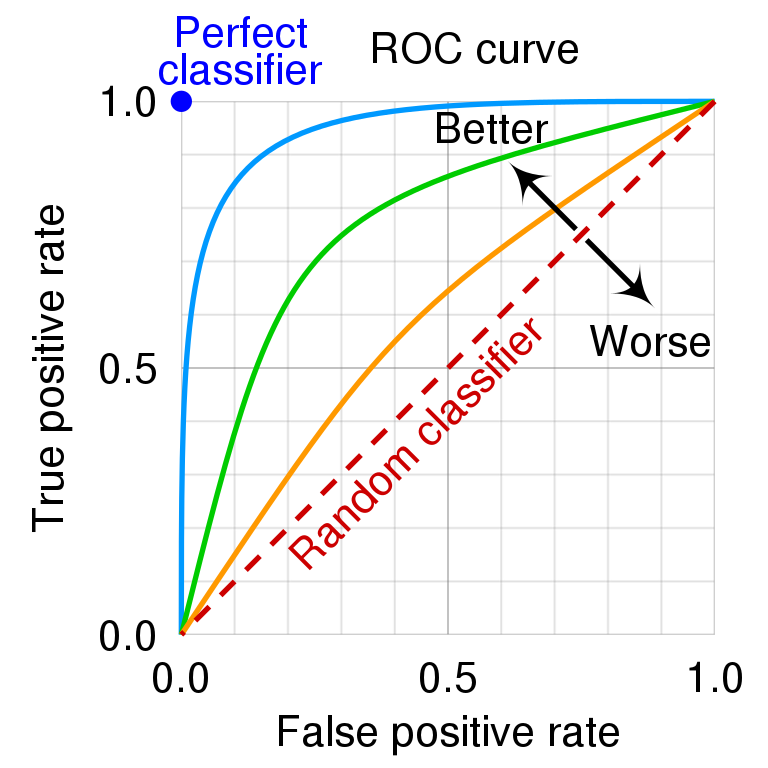
\includegraphics[width=4cm,height=4cm]{generative-models/roc-curve.png}
    \end{figure}} 
    \begin{itemize} \footnotesize
        \item An ideal ROC curve will hug the top left corner. \pause
        \item The larger the AUC the better the classifier.
    \end{itemize}

\end{columns}


\end{frame}



\subsection{Quadratic discriminant analysis}
\begin{frame}{Quadratic discriminant analysis}
    \begin{itemize}
        \item Assumes that the discriminant observations from each class are drawn from a \textbf{Gaussian distribution}. \pause 
        
        \item The idea is to compute each estimate and then plug them Bayes' theorem in order to perform a prediction. \pause 

        \item However, QDA assumes that each class has its \textbf{own covariance matrix}. \pause 
        
        \\ $\rightarrow$ Assumes that an observation from the $k$th class is of the form $X \sim N (\mu_k , \Sigma_k )$, where $\Sigma_k$ is a covariance matrix for the $k$th class. \pause 

        \item Under this assumption, the Bayes classifier assigns an observation $X = x$ to the class for which \pause 

        \begin{equation}\label{eq:delta-quatratic}
            \delta_k = - \frac{1}{2} x^T \Sigma_{k}^{-1} x + x^T \Sigma_{k}^{-1} \mu_k - \frac{1}{2} \mu_k^T \Sigma_{k}^{-1} \mu_k - \frac{1}{2} \log{|\Sigma_{k}|} + \log{\pi_k}
       \end{equation} 

       is largest. \pause 

        \item So the QDA classifier involves plugging estimates for $\mu_k , \Sigma_k$ and $\pi_k$ into (\ref{eq:delta-quatratic}), and then assigning an observation $X = x$ to the class for which this quantity is \textbf{largest}.
        
    \end{itemize}
\end{frame}



\subsection{When to use Linear vs quadratic discriminant analysis?}
\begin{frame}{When to use Linear vs quadratic discriminant analysis?}



\begin{columns}[T]
\column{0.5\linewidth}
  \textbf{With linear discriminant analysis: }
    \begin{itemize}
        \item<1-> Assumes common covariance matrix and becomes linear in $x$, for a total of \textcolor{blue}{$Kp$} linear coefficients to estimate. 

        \item<3-> LDA is a much less flexible classifier. 

        \item<5-> LDA can suffer from high bias.

    \end{itemize}


    \column{0.5\linewidth}
   \textbf{With quadratic discriminant analysis:}
    \begin{itemize}
        \item<2->Estimates a separate covariance matrix for each class, for a total of \textcolor{blue}{$Kp(p+1)/2$} parameters. 

        \item<4-> Recommended if the training set is very large, so that the variance is not a major concern. 
        
        \item<6-> Use it when the assumption of a common covariance matrix is clearly untenable.
    \end{itemize}
\end{columns}

\end{frame}


\subsection{Naive Bayes}
\begin{frame}{Naive Bayes}{Introduction}
    \begin{itemize}
    
        \item Recall that Bayes’ theorem provides an expression for the posterior probability, $p_k(x) =  \text{Pr}(Y=k|X=x)$ in terms of $\pi_1 , \cdots , \pi_K$ and $f_1(x), \cdots , f_K(x)$. \pause

        \begin{equation*}
           p_k(x) =  \text{Pr}(Y=k|X=x) = \frac{\pi_k f_k (x)}{  \sum_{l=1}^K \pi_l f_l(x)  }. 
        \end{equation*} \pause
        
        \item As we saw in previous sections, estimating the prior probabilities $\pi_1 , \cdots , \pi_K$ is typically straightforward: for instance, we can estimate $\hat{\pi}_k$ as $\hat{\pi}_k = n_k / n$. \pause
        
        \item However, estimating $f_1(x), \cdots , f_K(x)$ is more subtle. \pause

        \item The naive Bayes classifier assumes, 

        \begin{equation}\label{eq:f-naive}
            f_k(x) = f_{k_1} (x_1) \times f_{k_2} (x_2) \times \cdots \times f_{k_p} (x_p)  
        \end{equation} \pause 
        
        where $f_{k_j}$ is the density function of the $j$th predictor among observations in the $k$th class. \pause  \textcolor{blue}{$\rightarrow$ Within the $k$th class, the $p$ predictors are independent. }
        
    \end{itemize}
\end{frame}

\begin{frame}{Naive Bayes}{Introduction}
    \begin{itemize}
        \item Once we have made the naive Bayes assumption, we can plug (\ref{eq:f-naive}) into (\ref{eq:bayes}) to obtain an expression for the posterior probability,

        \begin{equation}\label{eq:naive-prob}
            p_k(x) = \frac{\pi_k f_{k_1} (x_1) \times f_{k_2} (x_2) \times \cdots \times f_{k_p} (x_p)  }{  \sum_{l=1}^K \pi_l f_{l_1} (x_1) \times f_{l_2} (x_2) \times \cdots \times f_{l_p} (x_p)  }
        \end{equation} \pause

        for $k = 1, \cdots, K.$

        \item To estimate the one-dimensional density function $f_{kj}$ using training data $x_{1j} , \cdots, x_{nj} $, we have a few options.

    \end{itemize}


\end{frame}

\begin{frame}{Naive Bayes}{Estimating the density function}

\begin{enumerate}
    \item \textbf{$X_j$ is quantitative and parametric} \pause

    \begin{itemize}
        \item We can assume that $X_j | Y=k \sim N(\mu_{jk}, \sigma_{jk}^2).$ \pause 

        \\ $\rightarrow$ We assume that within each class, the $j$th predictor is drawn from a (univariate) normal distribution. \pause 

        \item But predictors are independent from each other. \pause  
        
        \\ $\rightarrow$ the class-specific covariance matrix is diagonal. \pause 
     \end{itemize}

    \item \textbf{$X_j$ is quantitative and non-parametric} \pause 

    \begin{itemize}
        \item A very simple way to do this is by making a histogram for the observations of the $j$th predictor within each class. \pause 
        \item Then, $f_{kj}(x_j)$ is the fraction of the training observations in the $k$th class that belong to the \textbf{same histogram bin} as $x_j$. \pause 
        \item Alternatively, we can use a \textit{kernel density estimator}, which is essentially a smoothed version of a histogram
    \end{itemize}

    \item \textbf{$X_j$ is qualitative}  \pause 
    \begin{itemize}
        \item Simply count the proportion of training  estimator observations for the $j$th predictor corresponding to each class. 
    \end{itemize}
    
\end{enumerate}


\end{frame}

